\chapter{Implementering}

I dette kapitel vil der blive lagt vægt på mere kode nære ting.



\section{Dialplan}

Til at bygge en dialplan er der lavet et bibliotek kaldet libdialplan, som står for at gemme og indlæse de dialplaner som brugeren laver ude i klienten, i en struktur der efterligner hvad brugeren ser, for nemt at kunne genindlæse en dialplan. Derfor har hvert komponent sin egen klasse i biblioteket, med en række felter svarende til de indstillinger som brugeren har for komponenten. Dette bibliotek genbruges i compileren, for dermed nemt at kunne indlæse den givende dialplan i typestærke elementer.


Når en dialplan er blevet bygget i klienten og gemt i databasen skal den skrives ned i det format som Freeswitch forstår og til det bruges compileren. Når et opkald kommer ind i PBX'en går det ind i en context kaldet public, derfra skal opkaldet så sendes ud til den rette reception. Derfor er det første som compileren laver, er at oprette en extension i public contexten hvorfra opkaldet bliver sendt ud til den pågældenes receptions context.
Ved at lave en context for hver reception, så giver det muligheden for at hvis der ikke er en extension der har alle sine conditions opfyldt og der ikke at lavet nogen anti-actions til at tage højde for det, så kan man fordi den leder fra top til bund, placere i bunden en extension hvor dens condition altid er opfyldt. Så hvis der for eksempel ikke er taget højde for et tidsinternal, så falder opkaldet til sidst altid ned i den. Det betyder så også at der kun kan være en per context.

\section{Server}

Når en forespørgelse kommer ind til webserver skal den først finde ud af hvilken resource som der spørges efter. Hvis serveren har en handler til den URL, bliver der først tjekket for om der er en token og om den gyldig. Hvis den er det bliver forespørgelse sendt videre til den rette controller. Spørges der f.eks. efter at få oprette en ny reception, bliver der spurt ind til Database for at få den oprettet og går det godt kommer der id'et på den nye reception tilbage, der så bliver sendt tilbage til klienten igen. 
Sådan opfører de fleste af controllerne sig.

\begin{figure}[ht!]
\centering
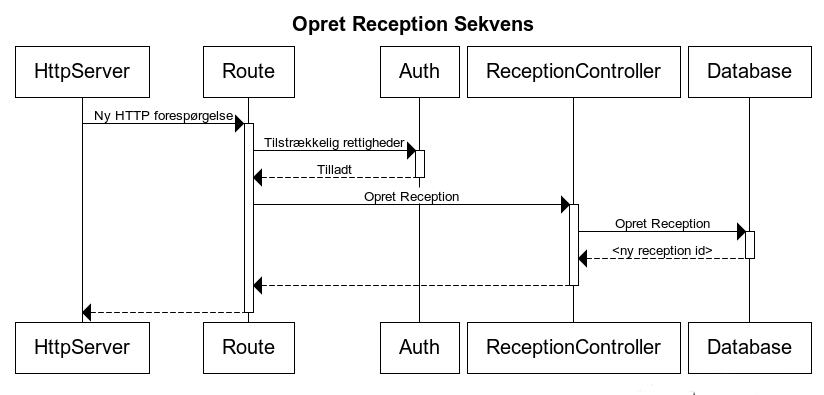
\includegraphics[width=\textwidth]{images/serversequence.png}
\caption{Når man kalder serveren for at oprette en ny reception}
\label{fig:serversequence}
\end{figure}

\pagebreak
\section{Migraring}
Når det nye system skal bruges er det vigtigt at kunne få det gamle data med over. Til det er der blevet skrevet et lille program. Programmet er skrevet i Dart fordi moddellen og forespørgelserne til database allerede var lavet i dart, hvilket gjorder det hurtigt at låne fra. Det gamle systems database var en Microsoft Access database og fordi at Dart ikke har support for at læse Access databaser blev der brugt et andet program mdb-export der gemmer tabellerne som komma seperaret filer. Migraringsprogrammet indlæser filerne til typestærke objekter og mapper det til felter i det nye database skema for så at gemme det i databasen.